\documentclass[
	%parspace, % Térköz bekezdések közé / Add vertical space between paragraphs
	%noindent, % Bekezdésének első sora ne legyen behúzva / No indentation of first lines in each paragraph
	%nohyp, % Szavak sorvégi elválasztásának tiltása / No hypenation of words
	%twoside, % Kétoldalas nyomtatás / Double sided format
	%final, % Teendők elrejtése / Set final to hide todos
]{elteikthesis}[2019/06/10]
\usepackage{tikz}
\usepackage{xcolor}
\usepackage{pgfplots}

\definecolor{bblue}{HTML}{4F81BD}
\definecolor{rred}{HTML}{C0504D}
\definecolor{ggreen}{HTML}{9BBB59}
\definecolor{ppurple}{HTML}{9F4C7C}

% Dolgozat metaadatai
% Document's metadata
\title{Automatikus zenei hangszerfelismerés többszólamú zenében mély neuronhálók segítségével} % cím / title
\date{2020} % védés éve / year of defense

% Szerző metaadatai
% Author's metadata
\author{Hamrák János}
\degree{programtervező informatikus MSc}

% Témavezető(k) metaadatai
% Superivsor(s)' metadata
\supervisor{Gombos Gergő} % belső témavezető neve / internal supervisor's name
\affiliation{Adjunktus, PhD} % belső témavezető beosztása / internal supervisor's affiliation
%\extsupervisor{Külső Kornél} % külső témavezető neve / external supervisor's name
%\extaffiliation{informatikai igazgató} % külső témavezető beosztása / external supervisor's affiliation

% Egyetem metaadatai
% University's metadata
\university{Eötvös Loránd Tudományegyetem} % egyetem neve / university's name
\faculty{Informatikai Kar} % kar neve / faculty's name
\department{Programozáselmélet és Szoftvertechnológiai\\ Tanszék} % tanszék neve / department's name
\city{Budapest} % város / city
\logo{elte_cimer_szines} % logo

% Irodalomjegyzék hozzáadása
% Add bibliography file
\addbibresource{thesis.bib}

% A dolgozat
% The document
\begin{document}
	
% Nyelv kiválasztása
% Set document language
\documentlang{magyar}
%\documentlang{english}


% Dokumentum beállítások
% Some document settings
% Lábjegyzet folytonos számozása fejezetek között
% Contiunous counting of footnotes among chapters
\counterwithout{footnote}{chapter}

% Tartalomjegyzék oldalszámozásának rejtése
% Hide page numbering of ToC
\newcounter{conpageno}
\let\oldtableofcontents\tableofcontents
\renewcommand{\tableofcontents}{
	\pagenumbering{gobble}
	\oldtableofcontents
	\cleardoublepage
	\setcounter{conpageno}{\value{page}}
	\pagenumbering{arabic}
	\setcounter{page}{\value{conpageno}}
}


% Címlap (kötelező)
% Title page (mandatory)
\maketitle
\topicdeclaration

% Tartalomjegyzék (kötelező)
% Table of contents (mandatory)
\tableofcontents
\cleardoublepage

% Tartalom
% Main content
\chapter{Bevezetés} % Introduction
\label{ch:intro}

Napjainkban a zenéhez legkönnyebben digitális formában, a világhálón keresztül férhetünk hozzá. Néhány kattintással olyan zenei tartalomszolgáltatókat érhetünk el, melyek széleskörű adatbázissal rendelkeznek. A folyamatosan bővülő adatmennyiség ellenére ezeknek az adatbázisoknak átláthatónak és könnyen kezelhetőnek kell maradniuk, hogy a felhasználókat a kívánt módon tudják kiszolgálni. Ennek érdekében nap mint nap új  megoldások születnek zenei információk automatikus kinyerése és feldolgozása céljából. Ezek teszik lehetővé a digitálisan tárolt zenék körében például az osztályozást vagy keresést.

A zenei információk kinyerésének tudományába (Music Information Retrieval, a továbbiakban: ''MIR'') tartozik a továbbiakban taglalt probléma, az automatikus hangszerfelismerés. Ez egy osztályozási feladat. Célja, hogy a meglévő digitális hanganyag alapján az adott zenéről megállapítsuk, hogy milyen hangszerek szólalnak meg benne. Ezt az információt több célra is fel tudjuk használni, például:
\begin{itemize}
 \item Későbbi feldolgozásra, további MIR feladatok inputjaként
 \item Statisztikák készítésére
 \item Adatbázisban való keresés szűrőfeltételeként
 \item Egy ajánlórendszer részeként, ahol az aktuális zeneszámot követően például egy hangszerelésében hasonló számot szeretnék ajánlani a felhasználónak.
\end{itemize}

Az automatikus hangszerfelismerés feladatot több aspektusból lehet megközelíteni, például a bemeneti adatok jellege, reprezentációja, a megvalósított architektúra, az osztályozás módszere, vagy az osztályok száma alapján. A dolgozatom keretein belül felkutatok néhány létező megoldást, majd ezekre alapozva prezentálom saját megközelítésemet és ennek eredményeit. Az általam bemutatott megoldás egy multi-label osztályozást valósít meg mély neuronhálós rendszer segítségével többszólamú zenében.

\section{Motiváció}

Az ember kognitív képességei segítségével a zenében könnyedén fel tudja ismerni az egyes hangszereket. Ugyanez a feladat a számítógép számára azonban már sokkal kevésbé triviális. Ennek egyik oka, hogy egy hangszer megszólaltatásának digitális reprezentációja nagyon változatos lehet. Függ például a hangszíntől, hangmagasságtól, hangerőtől és előadásmódtól, de a felvétel minőségétől és az esetleges háttérzajtól is. További nehezítő körülmény a többszólamúság, amikor egy időben több hangszert is megszólaltatunk, ezzel összemosva az egyszólamú környezetben is sokváltozós képünket.

A MIR nagyban támaszkodik a mesterséges intelligenciára. A számítógépek számítási kapacitásának folyamatos növekedése és az elérhető adathalmazok gyarapodása által pedig egyre nagyobb figyelmet kap a mesterséges intelligencia egy kiemelten számításigényes részterülete: a mély tanulás. Ezt bizonyítja, hogy az évente megrendezésre kerülő ISMIR (International Society for Music Information Retrieval) konferencián 2010-ben még csak 2 (\cite{florian2010}, \cite{Hamel2010}) mély tanulással kapcsolatos cikk jelent meg, de 2015-ben már 6, 2016-ban pedig már 16. \cite{choi2017tutorial}

A mély tanulás tehát egy ígéretes módszer lehet a MIR problémák megoldásában, ideértve az automatikus hangszerfelismerést is. Ezt kihasználva és megoldás életszerűségére törekedve döntöttem úgy, hogy elkezdek kísérletezni mély neuronhálókkal többszólamú zenében. Célom volt találni egy tanításra alkalmas adathalmazt, azon pedig tervezni egy olyan mély neuronhálós rendszert, amely a jelenlegi megoldások pontosságát meghaladja.


\section{A dolgozat felépítése}

Dolgozatomban tehát az eddigi kapcsolódó kutatásokat, illetve saját munkám eredményét dolgozom fel. A következő alfejezetben felsorolom az általam relevánsnak tartott, a State-of-the-Arthoz vezető kutatásokat. 

A második fejezetben betekintést adok a téma elméleti hátterébe. Először kifejtem a zenével kapcsolatos főbb fogalmakat, bemutatom fontosabb tulajdonságait, reprezentációit. Kitérek a MIR bemutatására is. Ezután bevezetem a gépi tanulás és a mély tanulás fogalmát. 

A harmadik fejezet az adathalmazokról fog szólni. Itt előbb felsorolom az adathalmazok kiválasztásának szempontjait, majd minden felhasznált adathalmaznak ismertetem a főbb jellemzőit. 

A negyedik fejezetben a módszertanról ejtek szót. Itt kifejtésre kerülnek az adatok előfeldolgozási módszerei, az általam bemutaott mély tanulási architektúrák, illetve ezek megvalósításai.

Az ötödik fejezetben részletezem az általam végzett kisérleteket és ezek eredményeit. Ezeket összevetem egymással, illetve a releváns State-of-the-Art kutatásokkal.

A hatodik fejezetben összegzem a leírtakat, valamint továbbgondolom a kutatásomat, felvázolok néhány ötletet annak jövőjéről.


\section{Kapcsolódó munkák}

Az automatikus hangszerfelismerés témában a korábbi kutatások túlnyomó része a monofónikus, azaz egyhangszeres zenékkel foglalkozik. Martin és Kim \cite{Martin1998} mintafelismerési statisztikai technikája 1023 izolált hangjegy és 15 különböző hangszer között a hangszercsaládok felismerésében 90\%-os, egyéni hangszerek felismerésében pedig 70\%-os pontosságot produkált. Brown \cite{brown1999} a kepsztrális együtthatókat használta fel K-közép klaszterezési módszeréhez. Eronen és Klapuri \cite{eronenklapuri2000} széleskörű, spektrális és időbeli feature-halmaz segítségével - összesen 43 különböző feature felhasználásával - 81\%-os hangszer és 95\%-os hangszercsalád pontosságról számolt be. Deng \cite{deng2008} klasszikus zenei hangszerek tekintetében elemezte a különböző, gépi tanulási módszerekben használatos feature összeállításokat. Bhalke \cite{bhalke2015} tört Fourier-transzformáción alapuló MFCC feature-ök segítségével tervezett CPNN osztályozót mutatott be, amellyel hangszercsaládok tekintetében 96.5\%-os, hangszerek tekintetében pedig 91.84\%-os pontosságot ért el.

Többszólamú környezetbe való átültetéssel foglalkozott Burred tanulmánya \cite{burred2010}, aki a többszólamúságot két kísérlettel közelítette meg. Először csak egy-egy hangjegyet kombinált össze többszólamú hangjeggyé. Itt két szimultán hangjegy esetén 73.15\%-os, három hangjegyre 55.56\%-os, négy hangjegy kombinációjára pedig 55.18\%-os pontosságot sikerült elérni. Másik kísérletként hosszabb szekvenciákat kombináltak össze, ekkor két hang esetén 63.68\%-os, három hang esetén pedig 56.40\%-os pontosságot kaptak. 

Eggink és Brown \cite{egginkandbrown2003} a polifónikus zenékben a hiányzó adat elméletükkel próbálták feltárni az egyes hangszereket. Ennek lényege, hogy felderítették azon idő- és frekvenciabeli részeket a zenén belül, ahol szeparáltan egy hangszer tulajdonságait vélték felfedezni és ezt dolgozták fel. Erre a módszerre épített Giannoulis és Klapuri \cite{giannoulisandklapuri2013} kutatása is, és hasonló megközelítést alkalmazott Garcia \cite{garcia2011} is.
 
Jiang \cite{Jiang2013} egy többlépcsős megoldást mutat be. Első lépésben a hangszercsaládot határozták meg, ezzel szűkítve a a lehetséges hangszerek halmazát és a változók számát. A pontos hangszer-meghatározás csak ezután következett.

Az előbbi kutatások többnyire hagyományos gépi tanulási megoldásokat alkalmaztak, amelyekhez maguk nyerték ki a különböző bemeneti feature-öket. Humphrey \cite{humphrey2012} írásában a mély tanulási architektúrákat ismerteti a MIR terület korszerű irányzataként. A témában gyakorlati segítségként szolgál Choi \cite{Choi2017} írása, amiben konkrét adatreprezentációkat, mély neuronhálós rétegeket, és mély tanulási technikákat mutat be.

Li \cite{li2015automatic} a nyers hanganyagot inputként felhasználva egy konvolúciós mély neuronhálós rendszert mutatott be a polifónikus zenében való automatikus hangszerfelismerés kapcsán. Ezt a megoldást aztán összevetette hagyományos gépi tanulási módszerekkel is. A mély neuronhálós rendszer teljesített legjobban. 75.60\%-os pontossággal, 68.88\%-os felidézéssel, 72.08 mikro F értékkel és 64.33 makro F értékkel. Han \cite{han2016deep} szintén egy mély konvolúciós hálót használt, azonban az osztályozás szempontjából máshogyan járt el: a zenékben egy darab domináns hangszert keresett. Bemenetként a zenék spektogramját használta fel, 0.602-es mikro és 0.503-as makro F értéket ért el.
\cleardoublepage


\chapter{Elméleti háttér} 
\label{ch:theory}

Ebben a fejezetben a dolgozathoz kapcsolódó fogalmakat és elméleti alapokat mutatom be. Először magának a zenének a releváns tulajdonságait mutatom be. Ezután ismertetem a MIR kutatási területet, amelybe dolgozatom is tartozik. Majd végül a mesterséges intelligencián alapuló megoldásokról nyújtok elméleti bevezetőt, érintve a hagyományos gépi tanulás és a mély tanulás módszereit is.

\section{Zene és reprezentációi} 

\subsection{Zene fogalma, tulajdonságai}

A zene egy meglehetősen összetett fogalom. Az ember számára a zene megjelenhet hang formájában, leírhatjuk őket szimbólumok segítségével egy kottában, előfordulhat szöveges formában dalszövegként, képi formában egy albumborító, vagy egy zenész képében, illetve mozdulatokban egy zenei előadás keretében. 

Often music means the audio content, although otherwise its scope extends to other types of musical infor-
mation e.g., lyrics, music metadata, or user listening history.

\subsection{Hang reprezentációk}

A hangok fizikai mivoltukban rezgésekként jelennek meg. A rezgéseket matematikailag olyan folytonos függvényekkel tudjuk leírni, melyek értelmezési tartománya az idő, értékkészlete pedig a nyugalmi állapothoz viszonyított pillanatnyi kitérés. Ilyen lehet például egy szinuszgörbe. Ahhoz, hogy a hangokat számítógépen tudjuk tárolni és feldolgozni, ezeket a függvényeket kell ábrázolnunk.  Mivel azonban a számítógép számábrázolása véges, ezért a hangokat először digitalizálni kell. Ez azt jelenti, hogy a folytonos függvényeket diszkrét, azaz véges helyen vett és véges értékekkel rendelkező fügvényekké alakítjuk. Ez úgy történik, hogy ez eredeti függvényünkből megadott időközönként mintát veszünk, diszkrét értékre kerekítjük, és ezeket az értékeket összefűzzük. Az így kapott függvény lesz a hang digitális reprezentációja.

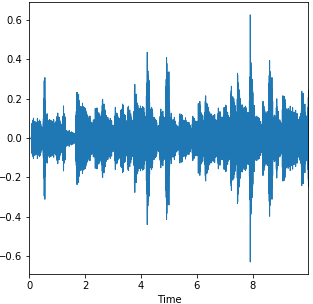
\includegraphics{wave.png}

A hangok digitális reprezentációja tehát lényegében egydimenziós, mivel egy függvénygörbének tekinthetjük. Ezt szokták hívni nyers hangnak is, ugyanis további reprezentációkká tudjuk transzformálni. A MIR területen megjelenő mély tanulási megoldások jelentős része ezen nyers hangábrázolás helyett inkább a kétdimenziós reprezentációkat alkalmazza bemenetként. Ezt azzal indokolják, hogy a nyers bemeneten való tanítás sikeréhez nagyobb adathalmaz szükséges, mint a kétdimenziós reprezentációkéhoz. \cite{Choi2017}



\subsection{Music Information Retrieval (MIR)} 

A bevezetőben már említettem a zenei információk kinyerését (music information retrieval - MIR). Ez egy interdiszciplináris kutatási terület, magában hordozza többek között a zeneelmélet, pszichoakusztika, pszichológia, informatika, jelfeldolgozás és gépi tanulás tudományágakat. Céljára jól utal az elnevezése, zenékből szeretnénk releváns információt kinyerni, és ezeket felhasználni \cite{Choi2017}. A felhasználásra szerintem nagyon jó, életszerű példát ad Downie 2003-as cikkének \cite{Downie2003} bevezetője, amelyet a következőképp fordíthatunk le:

''Képzeljünk el egy világot, ahol egyszerűen felénekelhetjük egy számítógépnek a dalrészletet, ami már reggeli óta a fejünkben jár. A gép elfogadja a hamis énekünket, kijavítja, és azonnal javaslatot tesz arra, hogy éppen a ''Camptown Races'' című számra gondoltunk. Miután mi belehallgatunk a gép által talált számos relevánsnak tartott MP3 fájl egyikébe, elfogadhatjuk a gép javaslatát. Ezután elégedetten elutasíthatjuk a felajánlást, hogy az összes további létező verzióját is felkutassa a dalnak, ide értve a nemrég megjelent olasz rap verziót, vagy a skótdudás duettre írt kottát.''  \cite{Downie2003}

Figyeljük meg, hogy ez a hétköznapi eset mennyire össztett probléma. A következő feladatok jelennek meg:
\begin{itemize}
\item Az emberi éneklés, vagy dúdolás alapján hangfelismerés.
\item Hang alapú lekérdezés egy zenei adatbázisban az előbbi bemenettel.
\item Hangelemzés, feldolgozás, hogy a hamis hangokat ki tudjuk javítani, az esetleges háttérzajokat eltávolítsuk, illetve ha kell, a dallamból automatikusan kottát generáljunk.
\item Hasonlóságon alapuló keresés zenék között, hogy megtaláljuk a kívánt dalt az adatbázisban.
\item Zenei feldolgozások detektálása, hogy további verzióit is megtaláljuk egy adott dalnak.
\end{itemize}

MIR problémák definiálását több szempontból közelíthetjük meg. Choi cikke \cite{Choi2017} két tengelyre osztja fel a problémateret: szubjektivitás és eldöntési időmérték. A szubjektivitás tengelyen léteznek szubjektívebb feladatok, melyekre nincsenek egyértelmű válaszok. Ilyen lehet például a zene műfajának meghatározása. Objektívebb feladatoknak tekinthetjük azokat, melyek eredménye egyértelműen meghatárhozható, esetleg számszerűsíthető. Ide tartozik a hangszerfelismerés, vagy a tempó észlelés. \cite{Choi2017}

A másik tengely, az eldöntési időmérték aszerint sorolja be a feladatokat, hogy mekkora időegységeken értelmezhető egy becslés. Ez egy relatív mérték. Például a dallamfelismerés eldöntési időmértékére azt mondhatjuk, hogy alacsony, mert egy felismert dallam jó eséllyel nem fedi le az egész zenét. Másik kifejezéssel azt mondhatjuk, hogy ez egy időben változó, azaz dinamikus tulajdonság. Ellenben a tempó általában állandó értékű az egész zenében, így a teljes zeneszámot fel tudjuk címkézni egy adott tempóval. Erre azt mondjuk, hogy eldöntési időmértéke relatív magas, azaz ez egy statikus tulajdonsága a zenének.\cite{Choi2017}

A hangszerfelismerést tekinthetjük statikus, illetve dinamikus feladatnak is a probléma megközelítésének függvényében. Dinamikus, ha erős címkézést szeretnénk megvalósítani, tehát arra vagyunk kíváncsiak, hogy adott időpillanatban éppen milyen hangszerek szólalnak meg. Gyenge címkézés esetén viszont a feladat statikussá válik. Ebben az esetben az egész zenére vetítve szeretnénk címkéket kapni egyes hangszerek jelenlétével, vagy a többi hangszerrel szembeni dominanciájával kapcsolatban.

TODO több MIR feladat


\section{Machine learning, Deep Learning}

ML, DL elhelyezése, 5. pdfem

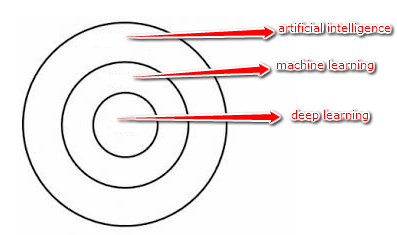
\includegraphics{ai.png}

\subsection{Machine Learning}

ML, ML in MIR

\subsection{Deep Learning}

DL, miben más mint az ML, architektúrák stb
\cleardoublepage

\chapter{Módszertan} 
\label{ch:methodology}

Ebben a fejezetben az alkalmazott módszertant mutatom be. Először ismertetem az alkalmazott előfeldolgozási módszereket. Ezután a tanító modellek architektúráját mutatom be. Végül pedig szót ejtek az ismertetett deep learning architektúrához tartozó hiperparaméterekről.

\section{Bemeneti adatok, előfeldolgozás}

Az OpenMIC adathalmazzal két formában kapjuk meg a bemeneti adatokat. Egyrészt elérhetőek a nyers hanganyagok .ogg formátumban. Másrészt rendelkezésre állt a VGGish nevű reprezentáció is, amelyről a \ref{subsec:VGGish}-es fejezetben írtam.

A bemeneti adatokat tanítás előtt néhány előfeldolgozási folyamaton vittem végig részben a megvalósíthatóság, részben pedig a performancianövelés érdekében. Ezekről írok a következő alfejezetekben.

\subsection{Alternatív reprezentációk kinyerése}

A .ogg fájlokból beolvasott nyers audioval való tanítás sajnos nem volt lehetséges, mivel ez egy memória szempontjából igen költséges reprezentáció, amihez a hardver eszközöm kapacitása kevésnek bizonyult. Helyette a dolgozat korábbi fejezetében bemutatott melspectogram és MFCC reprezentációkat használtam fel. Mindkét reprezentációt a beolvasott nyers hullámforma reprezentációból nyertem ki az elméleti háttér fejezetben leírt módon.

\subsection{Adathalmazok normalizálása}

Az adatok normalizálása a tanulási folyamat gyorsítására szolgál. A normalizálást úgy érjük el, hogy az adatokat arányosan a 0 és 1 értékek közé transzformáljuk. Erre egy szokásos megoldás:
\begin{equation}
x(_i) := (x(_i) - x_{\text{min}}) \/ (x_{\text{max}} - x_{\text{min}})
\end{equation}

A normalizált adathalmazon a gradiens általában hamarabb csökkenthető, ezért a tanítási folyamat rövidebb lehet. \cite{LeCun2012}

\subsection{Osztályok kiegyenlítése}

Tanító modelleknél gyakori probléma, hogy a tanulni kívánt osztályok egy része alulreprezentált. Dolgozatom multi-label osztályozása esetén két osztályról beszélhetünk: igaz (jelen van az adott hangszer) és hamis (nincs jelen az adott hangszer). Mivel sok esetben a hamis értékek jelentős többségben voltak - egyes hangszerek esetén az összes adat közel 80\%-át is kitette -, ezért a modell jó pontosságot tudott elérni csupán “hamis” predikciókkal.

Ezt elkerülendő, három megoldás jöhetett szóba:
\begin{itemize}
 \item \textbf{Alulmintavételezés (Undersampling)} - a többségi osztályokból véletlenszerűen eltávolítunk annyi elemet, hogy az osztályok kiegyensúlyozottá váljanak.
 \item \textbf{Túlmintavételezés (Oversampling)} - a kisebbségi osztályok véletlenszerű elemeit duplikáljunk addig, amíg az osztályok kiegyensúlyozottá válnak.
 \item \textbf{Adat augmentáció (Data augmentation)} - hasonlóan az oversampling technikához a kisebbségi osztály elemeit bővítjük. Ebben az esetben a meglévő elemek transzformálásával mesterségesen hozunk létre új elemeket (pl. képeknél forgatás). \cite{imbalanced}
\end{itemize}

Dolgozatom keretében az undersampling módszert alkalmaztam.

\subsection{Tanító, tesztelő, és validáló halmaz kialakítása}

Tanító modellek alkalmazásakor fontos, hogy legalább kettő, de inkább három független adathalmazzal rendelkezzünk: 
\begin{itemize}
 \item \textbf{Tanító adathalmaz (Train set)} - ebből a halmazból tanul, és ezt a halmazt látja a modellünk.
 \item \textbf{Validáló adathalmaz (Validation set)} - a tanítási lépések (epoch-ok) között ezen - a tanító halmaztól független - adathalmazon kiértékeljük modellünk működését. Ezáltal visszajelzést tudunk adni a tanítási folyamat felé, és ha szükséges, változtathatunk a hiperparamétereken. Modellünk tehát ezt a halmazt időnként látja, de nem ebből tanul.
 \item \textbf{Teszt adathalmaz (Test set)} - a tanítási folyamat végén ezen a halmazon értékeljük ki modellünk teljesítményét. Modellünk ezt a halmazt a tanítás alatt egyáltalán nem látja, és ezáltal nem is tud tanulni belőle. Ezzel a függetlenséggel biztosítjuk a kiértékelés torzítatlanságát. \cite{traintestvalid}
\end{itemize}

Bevett szokás, hogy az adathalmazunkat véletlenszerűen, körülbelül 60\%-20\%-20\% arányban felosztjuk a fent említett három diszjunkt halmazra úgy, hogy a nagyobb részt a tanító halmaz kapja. \cite{traintestvalid} Dolgozatom során én is ezt az elvet követtem.

\section{Architektúra}

A következő alfejezetekben a különböző tanító modell kísérletek architektúráját mutatom be.

\subsection{Hagyományos machine learning (Modeling Baseline)}

Az OpenMIC dataset megalkotói bemutattak egy példa modellt, amely egy véletlen erdő osztályozó (random forest classifier). \cite{humphrey2018openmic} Ez egy hagyományos gépi tanulási algoritmus. Az osztályozó 100 eldöntési fából áll, a maximális mélysége 8. Ez szolgált munkám kiinduló pontjaként. A továbbiakban Modeling Baseline elnevezéssel hivatkozok rá.

A Modeling Baseline futtatását alapvetően a VGGish reprezentációra implementálták. Dolgozatom keretében megvalósítottam ugyanennek az osztályozónak a melspectogram, illetve MFCC reprezentációkon való tanítását is. Ezáltal minden reprezentációra kaptam egy viszonyítási alapot.

\subsection{Deep CNN}

Az első mély tanulási megközelítésem a VGG-16 \cite{vgg} architektúrához hasonló mély konvolúciós neuronháló megvalósítása. Ennek megfelelően Deep CNN néven fogok rá hivatkozni a továbbiakban. A VGG-16 egy 2014-ben bemutatott architektúra, amelyet 224x224 méretű RGB képek tanítására hoztak létre. Több tanulmány is azt állítja, hogy az ehhez hasonló mély konvolúciós hálók hangok tanítására is alkalmasak lehetnek (például \cite{choi2017tutorial}). Erre az állításra az intuíció pedig az lehet, hogy a hangok különböző kétdimenziós reprezentációi képek, melyekben a mély konvolúciós hálók mintákat, összefüggéseket tudnak keresni.

\begin{figure}[H]
  \centering
  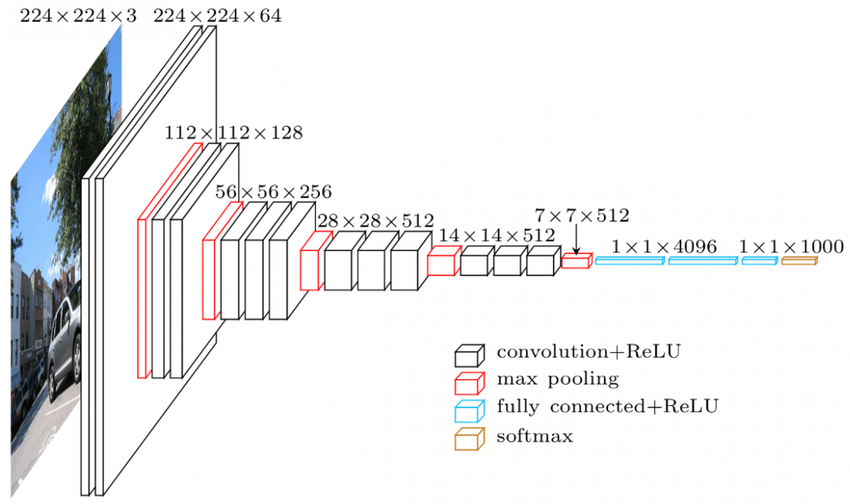
\includegraphics[width=\textwidth, height=8cm]{vgg.png}
  \caption{VGG-16 neurális háló architektúrája, forrás: \cite{loukadakis2018}}
\end{figure}

Az architektúra a következő elemekből épül fel:

\begin{itemize}
 \item konvolúciós rétegek, ReLU aktivációs függvénnyel
 \item max-pooling rétegek
 \item opcionálisan dropout rétegek
 \item flattening réteg
 \item teljesen kapcsolt rétegek, ReLU aktivációs függvénnyel
 \item teljesen kapcsolt utolsó réteg, szigmoid aktivációs függvénnyel
\end{itemize}

A bemenetet először két konvolúciós rétegnek adjuk át. Ezt követi egy max-pooling réteg, majd esetleg a nagyobb random-faktor érdekében egy dropout réteg. Ezután ugyanilyen sorrendben még háromszor-négyszer (attól függően, milyen mély architektúrát szeretnénk megvalósítani) hozzáfűzzük ezeket a rétegeket az előző kimenetéhez. Ahogy a konvulúciós rétegek zsugorodnak a max-poolingok hatásaként, úgy egyre több szűrővel érdemes ellátni őket. A következő egy flattening réteg, amely lehetőséget biztosít arra, hogy teljesen kapcsolt rétegeket csatoljunk utána. Dropout rétegeket itt is alkalmazhatunk. Az utolsó teljesen kapcsolt réteghez szigmoid aktivációs függvény tartozik, hogy 0 és 1 közötti értékeket kapjunk a kimenetre. Ebből nyerjük ki a végleges igaz-hamis értékeket.

Erre az architektúrára csak a melspectogram reprezentációt lehetett ráilleszteni. A VGGish 10 és az MFCC 20 méretű dimenziója a konvolúciók és összevonások következtében nulla alá redukálódott volna, ami nem lehetséges. Ezért ezen architektúrával a kísérlezetést abbahagytam, ezt egy későbbi kutatás során lehetne folytatni.

\begin{table}[H]
	\centering
	\begin{tabular}{ | c | c |}
		\hline
		\textbf{Réteg} & \textbf{Melspec}  \\
		\hline \hline
		\emph{Input} & 1 $\times$ 128 $\times$ 430 \\
		\hline
		\emph{Conv2D} & 64 $\times$ 128 $\times$ 430 \\
		\hline
		\emph{Conv2D} & 64 $\times$ 128 $\times$ 430 \\
		\hline
		\emph{MaxPool2D} & 64 $\times$ 63 $\times$ 214 \\
		\hline
		\emph{Dropout} & 64 $\times$ 63 $\times$ 214 \\
		\hline 
		\emph{Conv2D} & 128 $\times$ 63 $\times$ 214 \\
		\hline
		\emph{Conv2D} & 128 $\times$ 63 $\times$ 214 \\
		\hline
		\emph{MaxPool2D} & 128 $\times$ 31 $\times$ 106 \\
		\hline
		\emph{Dropout} & 128 $\times$ 31 $\times$ 106 \\
		\hline 
		\emph{Conv2D} & 256 $\times$ 31 $\times$ 106 \\
		\hline
		\emph{Conv2D} & 256 $\times$ 31 $\times$ 106 \\
		\hline
		\emph{MaxPool2D} & 256 $\times$ 15 $\times$ 52 \\
		\hline
		\emph{Dropout} & 256 $\times$ 15 $\times$ 52 \\
		\hline 
		\emph{Conv2D} & 512 $\times$ 15 $\times$ 52 \\
		\hline
		\emph{Conv2D} & 512 $\times$ 15 $\times$ 52 \\
		\hline
		\emph{MaxPool2D} & 512 $\times$ 7 $\times$ 25 \\
		\hline
		\emph{Flatten} & 89600 \\
		\hline
		\emph{Fully-connected} & 4096 \\
		\hline
		\emph{Fully-connected} & 2048 \\
		\hline
		\emph{Fully-connected} & 1 \\
		\hline
	\end{tabular}
	\caption{Deep CNN architektúra rétegei és az egyes rétegek outputjainak mérete melspectogram reprezentáció esetén}
	\label{tab:dcnn}
\end{table}

\subsection{Shallow CNN (Embedding downstream CNN)}

Kísérleteim során a Deep CNN után egy sekélyebb architektúrát is kialakítottam. Ezt a továbbiakban Shallow CNN néven fogom említeni. A Shallow CNN-t három okból hoztam létre:
 
\begin{itemize}
 \item Amint azt az adathalmazok körében a \ref{subsec:VGGish}-es alfejezetben is említettem, a VGGish reprezentáció már előre tanított, ezért erre nem lenne hatékony egy Deep CNN mélységű architektúra alkalmazása.
 \item A melspectogram, illetve MFCC reprezentációk esetében a kísérletek arra utaltak, hogy túl kevés az adatunk egy ilyen mély architektúra alkalmazásához. Az eredmények azt mutatták, hogy a modell fölöslegesen próbál nagyon mély összefüggéseket keresni az adatok között. Ezek feltárásához az adott ezres nagyságrendű bemeneti mintaszám helyett legalább tízezres, de inkább százezres kellene.
 \item Az MFCC és VGGish reprezentációk mérete nem megfelelő a megadott architektúra dimenzióredukciói miatt.
\end{itemize}

Maga a Shallow CNN a Deep CNN leegyszerűsített változata, tehát egy sekélyebb konvolúciós neuronháló megvalósítása. A rétegek típusa megegyezik a Deep CNN-ével, azonban számuk és méretük jelentősen kisebb (lásd \ref{tab:scnn} táblázat). Ennek eredményeképpen jelentősen csökkent a tanítási idő, a modell teljesítőképessége pedig nőtt.


\begin{table}[H]
	\centering
	\begin{tabular}{ | c | c | c | c |}
		\hline
		\textbf{Réteg} & \textbf{VGGish} & \textbf{MFCC} & \textbf{Melspec}  \\
		\hline \hline
		\emph{Input} & 1 $\times$ 10 $\times$ 128 & 1 $\times$ 20 $\times$ 430 & 1 $\times$ 128 $\times$ 430 \\
		\hline
		\emph{Conv2D} & 64 $\times$ 10 $\times$ 128 & 64 $\times$ 20 $\times$ 430 & 64 $\times$ 128 $\times$ 430 \\
		\hline
		\emph{Conv2D} & 64 $\times$ 10 $\times$ 128 & 64 $\times$ 20 $\times$ 430 & 64 $\times$ 128 $\times$ 430 \\
		\hline
		\emph{MaxPool2D} & 64 $\times$ 4 $\times$ 63 & 64 $\times$ 9 $\times$ 214 & 64 $\times$ 63 $\times$ 214 \\
		\hline
		\emph{Dropout} & 64 $\times$ 4 $\times$ 63 & 64 $\times$ 9 $\times$ 214 & 64 $\times$ 63 $\times$ 214 \\
		\hline 
		\emph{Conv2D} & 128 $\times$ 4 $\times$ 63 & 128 $\times$ 9 $\times$ 214 & 128 $\times$ 63 $\times$ 214 \\
		\hline
		\emph{MaxPool2D} & 128 $\times$ 1 $\times$ 31 & 128 $\times$ 4 $\times$ 106 & 128 $\times$ 31 $\times$ 106 \\
		\hline
		\emph{Dropout} & 128 $\times$ 1 $\times$ 31 & 128 $\times$ 4 $\times$ 106 & 128 $\times$ 31 $\times$ 106 \\
		\hline
		\emph{Flatten} & 3968 & 54272 & 420608 \\
		\hline
		\emph{Fully-connected} & 128 & 128 & 128 \\
		\hline
		\emph{Fully-connected} & 1 & 1  & 1 \\
		\hline
	\end{tabular}
	\caption{Shallow CNN architektúra rétegei és az egyes rétegek outputjainak mérete reprezentációtól függően}
	\label{tab:scnn}
\end{table}

\section{Hiperparaméterek}

Az előfeldolgozási technikákon és az architektúra kialakításán kívül fontos szerepe volt a megfelelő hiperparaméterek megválasztásának is. Ezek többségét best-practice-ek alapján határoztam meg, majd kísérletezések során optimalizáltam. A különböző hiperparaméterek:

\begin{itemize}
 \item \textbf{Tanulási ráta (Learning rate)} - a tanulás mértékét határozza meg. Túl magas érték esetén előfordul, hogy a modellünk nem tud konvergálni az optimális megoldás felé, mert folyton átugorja azt. Túl alacsony érték esetén pedig a tanítás folyamata túl hosszú lehet, illetve előfordulhat, hogy bizonyos nem kielégítő lokális minimum gradiens érték irányába konvergálunk, amelyet épp át kellene ugranunk az optimális megoldás megtalálásához.
 \item \textbf{Epoch-ok száma + early stopping} - a tanulásban az epoch-ok száma jelenti azt, hogy a modell hány alkalommal megy végig a bemeneti tanítóhalmazon. Ennek 50 értéket adtam és early stopping technikával egészítettem ki. Az early stopping lényege, hogy minden epoch után egy kiválaszott érték alapján megvizsgáljuk, hogy a tanulás még hatékony-e, és ha nem, akkor leállítjuk. Én ezt a tanulási ráta függvényében, magas tanulási ráta esetén 4, alacsony esetén 7 epoch türelmi küszöbbel a validációs hiba csökkenésének vizsgálatára alapozva vezettem be.
 \item \textbf{Dropout} - az architektúra egyes rétegei közé dropout rétegeket illesztettem, amelyek az adott rétegig beállított súlyok egy részét véletlenszerűen eldobják az overfitting jelenség elkerülése érdekében. Ezt bármely két réteg közé beilleszthetjük és bármilyen mértékű lehet. Én a súlyok 20\%-ára állítottam be őket, az architektúrában feltüntetett pontokon.
 \item \textbf{Mini-batch size} - ennek az értéke adja meg, hogy egy időben hány konkrét bemeneti adaton végezzük el a léptetési és visszacsatolási folyamatokat. Ez az érték bármi lehet egytől a bemeneti adataink számáig. Minél kisebb az érték, annál kevésbé memóriaigényes a tanítás, és minél nagyobb az érték, annál gyorsabb. Best-practice-ként alacsony kettő-hatványértékeket szokás használni. Ebből kiindulva én 64-nek választottam meg.
\end{itemize}
\cleardoublepage

\chapter{Adathalmaz}
\label{ch:dataset}

Ebben a fejezetben a munkám kapcsán felkutatott és alkalmazott adathalmazokról lesz szó. Egy deep learning megoldás tervezésének első lépéseként érdemes egy alkalmas kiinduló adathalmazt kiválasztani. Ezt aztán a modell tanítására és tesztelésre használjuk.

\section{Kiválasztási szempontok}

//TODO ismir dataset gyűjtemény
pl. többszólam, ingyenesen elérhető, szerteágazó (not biased), stb gyenge címkézés

\section{Philharmonia Orchestra}

Kutatásom első fázisában a Philharmonia Zenekar ingyenesen elérhető hangminta könyvtárát használtam fel. Ebben egyszólamú mintákat találunk. A minták a főkönyvtáron belül a bennük megszólaló hangszer nevével megegyező könytárban találhatóak, ez biztosítja a címkéket. 

//TODO tulajdonságai

\section{OpenMIC}

A többszólamúság bevezetését a kutatásomban az OpenMIC \cite{humphrey2018openmic} adathalmaz felhasználásával értem el.  
//TODO  openmic cikk alapján
\cleardoublepage

\chapter{Kísérletek, eredmények} 
\label{ch:results}

Ebben a fejezetben értékelem ki és vetem össze különböző kísérleteim eredményeit.

\section{Mérőszámok}

A modellek teljesítményét F értékek alapján vetettem össze, egyrészt hangszerenként külön-külön, másrészt a hangszerenkénti átlagot véve is. Az F értékhez a következő metrikák vezettek el:

\begin{itemize}
\item \textbf{Pontosság (Accuraccy)} - a modell helyes előrejelzéseinek száma osztva az összes előrejelzés számával. Ez már magában egy jó mérőszám tud lenni, azonban multi-label osztályozások esetén érdemes a helytelen előrejelzések fajtájával is kalkulálni. Ezek a valótlan igazak (false positives) és valótlan hamisak (false negatives).
\begin{figure}[H]
  \centering
  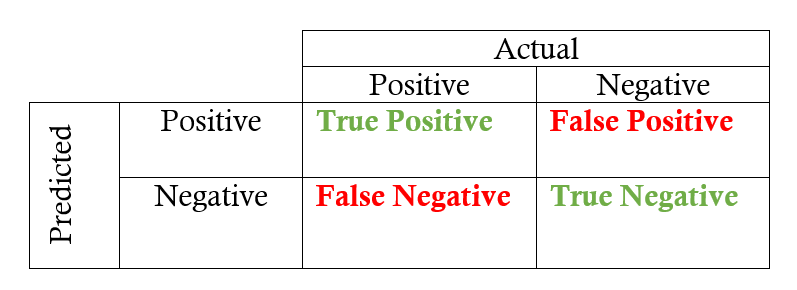
\includegraphics[width=\textwidth]{predictedactual.png}
  \caption{Előrejelzések fajtái, forrás: \cite{fscore}}
\end{figure}

\item \textbf{Veszteség (Loss)} - a veszteségfüggvény eredménye. A modell predikcióinak a valóságtól való eltérését összeadva kapjuk meg. A modell célja tanuláskor ennek az értéknek a minimalizálása.
\item \textbf{Precizitás (Precision)} - valós igaz predikációk száma osztva a valós és valótlan igazak számának összegével.
\item \textbf{Felidézés (Recall)} - valós igaz predikációk száma osztva a valós igaz és valótlan hamis predikációk összegével.
\begin{figure}[H]
  \centering
  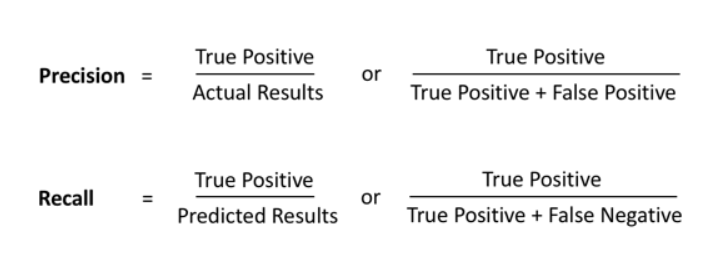
\includegraphics[width=\textwidth]{precisionrecall.png}
  \caption{Precizitás és felidézés, forrás: \cite{fscore}}
\end{figure}
\item \textbf{F érték (F score)} - a precizitás és felidézés értékek harmónikus közepe. Ez lesz tehát a meghatározó mérőszám modelljeink összevetésénél. \cite{fscore}

\begin{figure}[H]
  \centering
  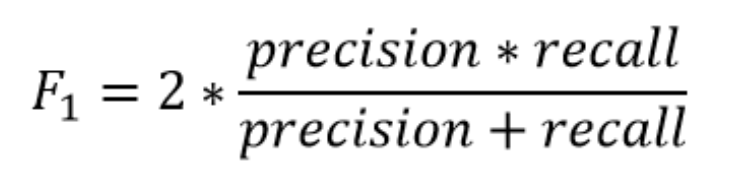
\includegraphics[width=6cm]{fscore.png}
  \caption{F score képlete, forrás: \cite{fscore}}
\end{figure}
\end{itemize}



\section{Eredmények}

A végső eredmények csak az OpenMIC datasettel kapcsolatos kísérleteket tartalmazzák. Az eredmények összevetésére a hangszerenkénti F score-okat használtam fel. Ez modellenként 19 hangszer, ami 19 különböző értéket jelent. Ezért minden modell végső összevetési alapjának két összesítő értéket választottam: az F-score-ok átlagát és a 0,70 feletti F score-t meghaladó hangszerek számát. Utóbbira a továbbiakban jól tanított hangszerként fogok hivatkozni. Saját intuícióm vezetett arra a következtetésre, hogy 0,70-es F score felett már életszerűen használható értékről beszélhetünk.

A továbbiakban a Modeling Baseline és a Shallow CNN architektúrák különböző eredményeit mutatom be.

\subsection{VGGish kiindulás}

Először a VGGish reprezentáció tekintetében tettem kísérleteket, mivel a Modeling Baseline eredeti implementációja ezt használta fel. Első lépésként ezt futtattam módosítás nélkül, majd lecseréltem a felhasznált RFC-t a saját CNN architektúrámra.

Az eredmények hangszerenként a \ref{fig:vggishbase} ábrán láthatóak. Az F-score-ok átlaga és a jól tanított hangszerek száma kicsivel magasabb volt a Modeling Baseline modellen, mint a Shallow CNN-en. Előbbi 0,79 átlag F score-t és 17 jól tanított hangszert, utóbbi 0,76 átlag F score-t és 14 jól tanított hangszert produkált.

\begin{figure}[H]
\centering
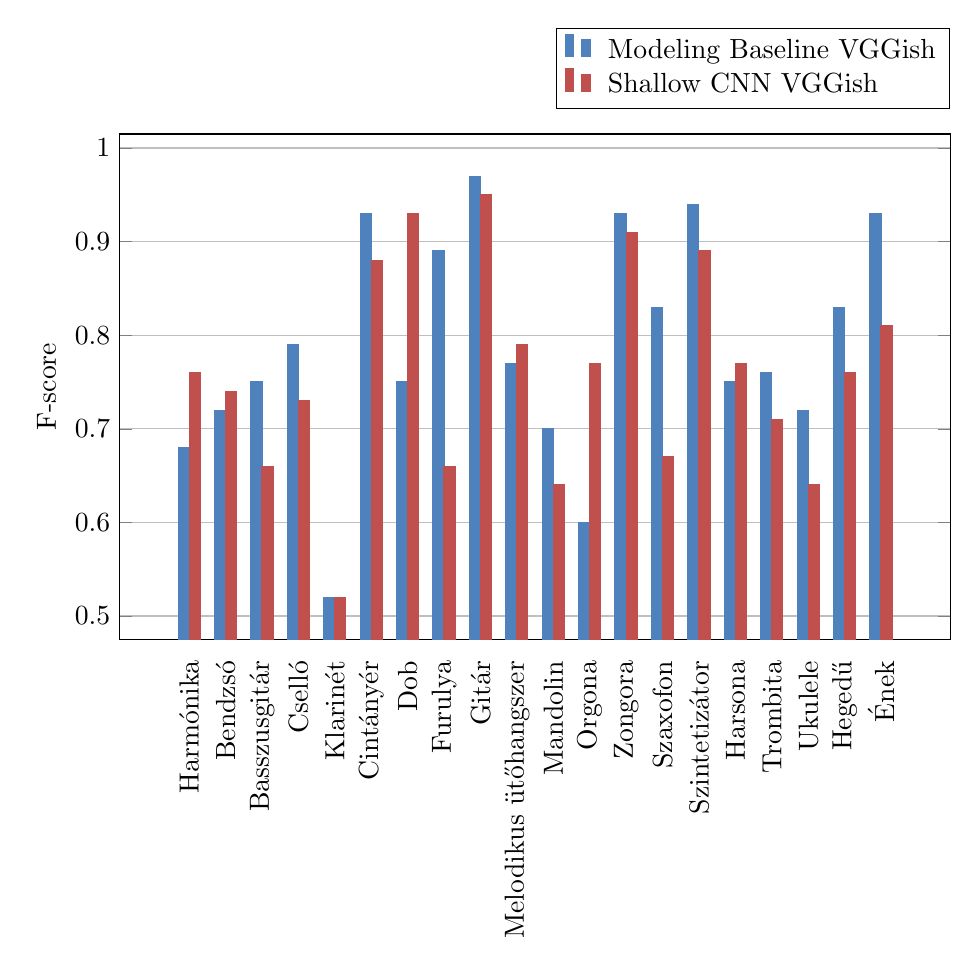
\begin{tikzpicture}
    \begin{axis}[
        width  = \textwidth,
        height = 8cm,
        major x tick style = transparent,
        ybar=0pt,
        bar width=4pt,
        ymajorgrids = true,
        ylabel = {F-score},
        symbolic x coords={Harmónika,Bendzsó,Basszusgitár,Cselló,Klarinét,Cintányér,Dob,Furulya,Gitár,Melodikus ütőhangszer,Mandolin,Orgona,Zongora,Szaxofon,Szintetizátor,Harsona,Trombita,Ukulele,Hegedű,Ének},
        xtick = data,
        x tick label style={rotate=90},
        scaled y ticks = false,
        legend cell align=left,legend style={
                at={(1,1.05)},
                anchor=south east,
                column sep=1ex}
    ]
        \addplot[style={bblue,fill=bblue,mark=none}]
            coordinates {(Harmónika, 0.68) (Bendzsó,0.72) (Basszusgitár,0.75)  (Cselló,0.79)  (Klarinét,0.52)  (Cintányér,0.93)  (Dob,0.75)  (Furulya,0.89)  (Gitár,0.97)  (Melodikus ütőhangszer,0.77)  (Mandolin,0.70)  (Orgona,0.60) (Zongora,0.93) (Szaxofon,0.83) (Szintetizátor,0.94) (Harsona,0.75) (Trombita,0.76) (Ukulele,0.72) (Hegedű,0.83) (Ének,0.93)};
        \addplot[style={rred,fill=rred,mark=none}]
            coordinates {(Harmónika, 0.76) (Bendzsó,0.74) (Basszusgitár,0.66) (Cselló,0.73) (Klarinét,0.52)  (Cintányér,0.88) (Dob,0.93) (Furulya,0.66) (Gitár,0.95)  (Melodikus ütőhangszer,0.79)  (Mandolin,0.64)  (Orgona,0.77) (Zongora,0.91) (Szaxofon,0.67) (Szintetizátor,0.89) (Harsona,0.77) (Trombita,0.71) (Ukulele,0.64) (Hegedű,0.76) (Ének,0.81)};
        \legend{Modeling Baseline VGGish ,Shallow CNN VGGish}
    \end{axis}
\end{tikzpicture}
\caption{Modeling Baseline és Shallow CNN kezdeti értékei optimalizációk nélkül VGGish reprezentáción} \label{fig:vggishbase}
\end{figure}


Ami még a \ref{fig:vggishbase} diagramról leolvasható, hogy a hangszerek között vannak jobban és kevésbé taníthatóak. Például a klarinét és mandolin mindkét modellen relatív alacsony F-értéket hozott. Ezzel szemben a gitár és zongora tanítása mindkét modell esetében 0.9 feletti F-értéket eredményezett.

A hangszereket vizsgálva a modellek között megjelentek nagyon hasonló és különböző értékek is. A legangyobb különbséget a Shallow CNN javára a dob mutatta, itt 0,75 állt szemben 0,93 értékkel, ami 0,18 F-score eltérés. A Modeling Baseline javára pedig a furulyával kapcsolatos számok jelentették a legnagyobb, 0,23 F-score eltérést. Itt 0,66 és 0,89 voltak az értékek.

\subsection{Optimalizáció}

Következő lépésként implementáltam a különböző előfeldolgozási adatoptimalizáló technikákat, mint például undersampling és normalizálió. Ezután szintén a VGGish reprezentáción futtatva a modellek teljesítménye javulást ért el: mindkét modell F score átlaga egyaránt 0,83-ra növekedett a korábbi 0,79-ről és 0,76-ról. Ezen felül a jól tanított hangszerek száma mindkét modell esetén elérte a maximális 20-at a korábbi 17 és 14 helyett. Ez a ShallowCNN számára magasabb relatív javulást jelent, ennek hangszerenkénti összevetése a \ref{fig:shallowcnnopt} ábrán látható.

\begin{figure}[H]
\centering
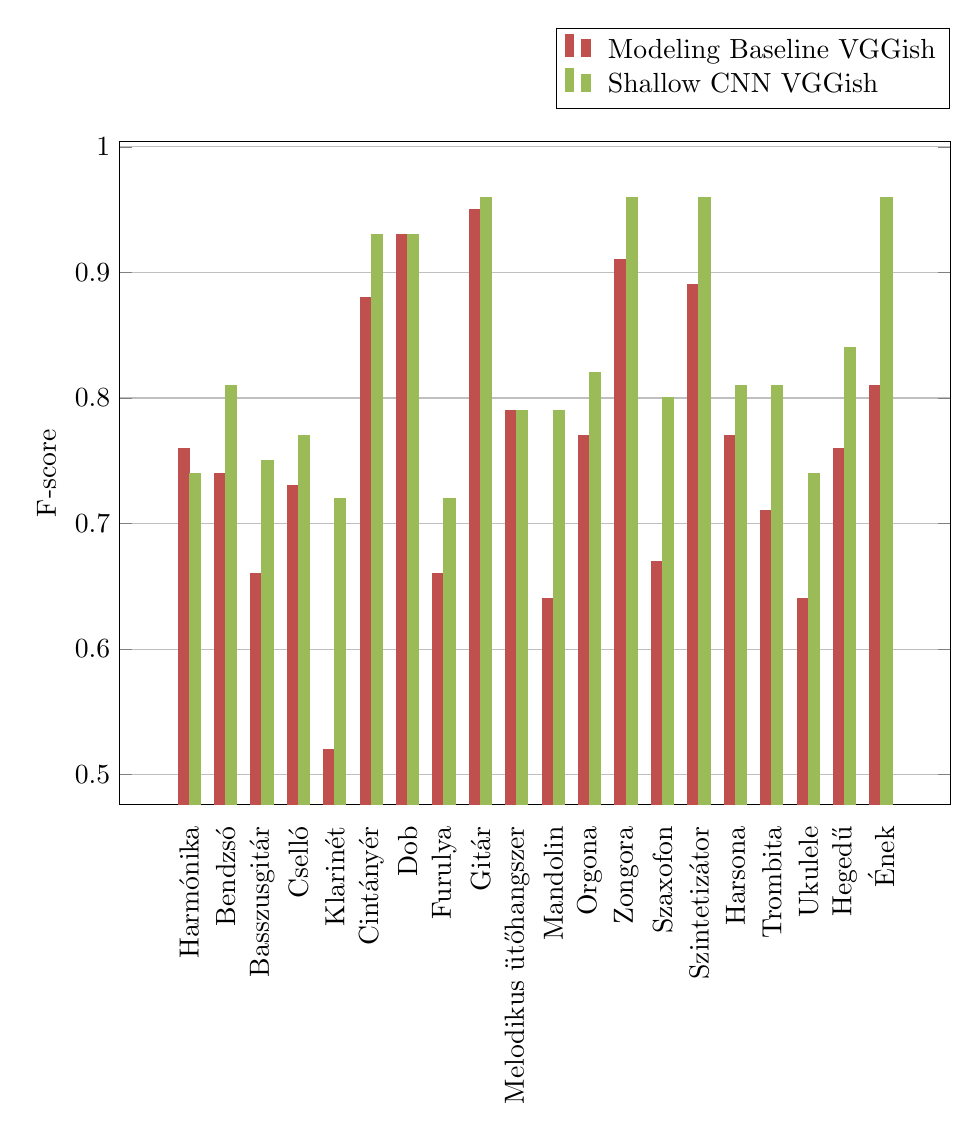
\begin{tikzpicture}
    \begin{axis}[
        width  = \textwidth,
        height = 10cm,
        major x tick style = transparent,
        ybar=0pt,
        bar width=4pt,
        ymajorgrids = true,
        ylabel = {F-score},
        symbolic x coords={Harmónika,Bendzsó,Basszusgitár,Cselló,Klarinét,Cintányér,Dob,Furulya,Gitár,Melodikus ütőhangszer,Mandolin,Orgona,Zongora,Szaxofon,Szintetizátor,Harsona,Trombita,Ukulele,Hegedű,Ének},
        xtick = data,
        x tick label style={rotate=90},
        scaled y ticks = false,
        legend cell align=left,legend style={
                at={(1,1.05)},
                anchor=south east,
                column sep=1ex}
    ] 
        \addplot[style={rred,fill=rred,mark=none}]
            coordinates {(Harmónika, 0.76) (Bendzsó,0.74) (Basszusgitár,0.66) (Cselló,0.73) (Klarinét,0.52)  (Cintányér,0.88) (Dob,0.93) (Furulya,0.66) (Gitár,0.95)  (Melodikus ütőhangszer,0.79)  (Mandolin,0.64)  (Orgona,0.77) (Zongora,0.91) (Szaxofon,0.67) (Szintetizátor,0.89) (Harsona,0.77) (Trombita,0.71) (Ukulele,0.64) (Hegedű,0.76) (Ének,0.81)};
       \addplot[style={ggreen,fill=ggreen,mark=none}]
            coordinates {(Harmónika, 0.74) (Bendzsó,0.81) (Basszusgitár,0.75) (Cselló,0.77) (Klarinét,0.72)  (Cintányér,0.93) (Dob,0.93) (Furulya,0.72) (Gitár,0.96)  (Melodikus ütőhangszer,0.79)  (Mandolin,0.79)  (Orgona,0.82) (Zongora,0.96) (Szaxofon,0.8) (Szintetizátor,0.96) (Harsona,0.81) (Trombita,0.81) (Ukulele,0.74) (Hegedű,0.84) (Ének,0.96)};
        \legend{Modeling Baseline VGGish ,Shallow CNN VGGish}
    \end{axis}
\end{tikzpicture}
\caption{Shallow CNN optimalizációk előtt és után VGGish reprezentáción} \label{fig:shallowcnnopt}
\end{figure}

\subsection{Alternatív reprezentációk}

//TODO MELSPEC, MFCC bevezetése, miért alacsonyabbak a számok, ml vs dl

\begin{figure}[H]
\centering
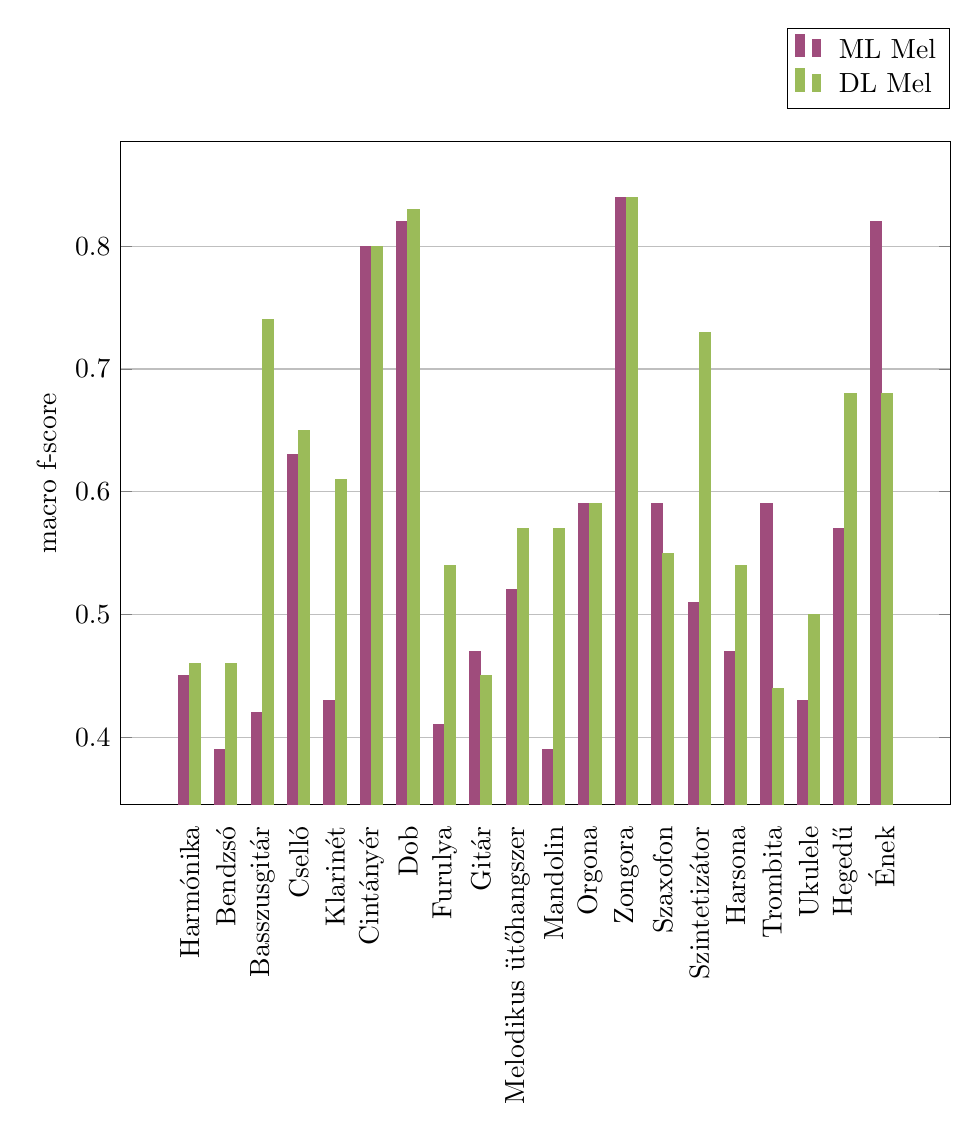
\begin{tikzpicture}
    \begin{axis}[
        width  = \textwidth,
        height = 10cm,
        major x tick style = transparent,
        ybar=0pt,
        bar width=4pt,
        ymajorgrids = true,
        ylabel = {macro f-score},
        symbolic x coords={Harmónika,Bendzsó,Basszusgitár,Cselló,Klarinét,Cintányér,Dob,Furulya,Gitár,Melodikus ütőhangszer,Mandolin,Orgona,Zongora,Szaxofon,Szintetizátor,Harsona,Trombita,Ukulele,Hegedű,Ének},
        xtick = data,
        x tick label style={rotate=90},
        scaled y ticks = false,
legend cell align=left,legend style={
                at={(1,1.05)},
                anchor=south east,
                column sep=1ex
        }
    ]
        \addplot[style={ppurple,fill=ppurple,mark=none}]
            coordinates {(Harmónika,0.45) (Bendzsó,0.39) (Basszusgitár,0.42) (Cselló,0.63)  (Klarinét,0.43)  (Cintányér,0.80)  (Dob,0.82)  (Furulya,0.41)  (Gitár,0.47)  (Melodikus ütőhangszer,0.52)  (Mandolin,0.39)  (Orgona,0.59) (Zongora,0.84) (Szaxofon,0.59) (Szintetizátor,0.51) (Harsona,0.47) (Trombita,0.59) (Ukulele,0.43) (Hegedű,0.57) (Ének,0.82) };

        \addplot[style={ggreen,fill=ggreen,mark=none}]
            coordinates {(Harmónika,0.46) (Bendzsó,0.46) (Basszusgitár,0.74) (Cselló,0.65)  (Klarinét,0.61)  (Cintányér,0.80)  (Dob,0.83)  (Furulya,0.54)  (Gitár,0.45)  (Melodikus ütőhangszer,0.57)  (Mandolin,0.57)  (Orgona,0.59) (Zongora,0.84) (Szaxofon,0.55) (Szintetizátor,0.73) (Harsona,0.54) (Trombita,0.44) (Ukulele,0.50) (Hegedű,0.68) (Ének,0.68) };
 	
        \legend{ML Mel,DL Mel}
    \end{axis}
\end{tikzpicture}
\caption{Modeling Baseline és Shallow CNN elődjének kezdeti értékei optimalizációk nélkül melspectogram reprezentáción} \label{fig:vggishbase}
\end{figure}
\cleardoublepage

\chapter{Összegzés, kitekintés} % Conclusion
\label{ch:sum}

Továbbfejlesztési ötletek:
//TODO undersampling helyett oversampling vagy data augmentation
cnn helyett rnn 
early stopping mellé model checkpoint
\cleardoublepage

% Irodalomjegyzék (kötelező)
% Bibliography (mandatory)
\addcontentsline{toc}{chapter}{\biblabel}
\printbibliography[title=\biblabel]
\cleardoublepage


\end{document}
